\chapter{Literature Review}
\label{2}
\section{Microfluidic Platforms for Lab-on-a-chip Applications}
\label{2_1}
Microfluidic platforms are defined with inner dimensions up to some hundreds of micrometers, and the microstructures inside microfluidic platforms have high surface-to-volume ratio. This provides more contact area to the channel walls for the fluid in the microchannels and this is helpful for the analysis of the near-wall micro-processes such as bacteria adhesion to surfaces. Furthermore, due to the decrease of physical dimensions microfluidic platforms also consume less fluid volumes and provide faster analysis and response times, which leads to lower cost and higher efficiency. Therefore microfluidic platforms are widely used for lab-on-a-chip applications in the field of biology procedures such as DNA analysis \cite{burns1998integrated}. Especially an emerging application area is integrating biochips into a microfluidic platform for clinical pathology like immediate point-of-care diagnosis of diseases.

\begin{figure}[ht]%
\centering
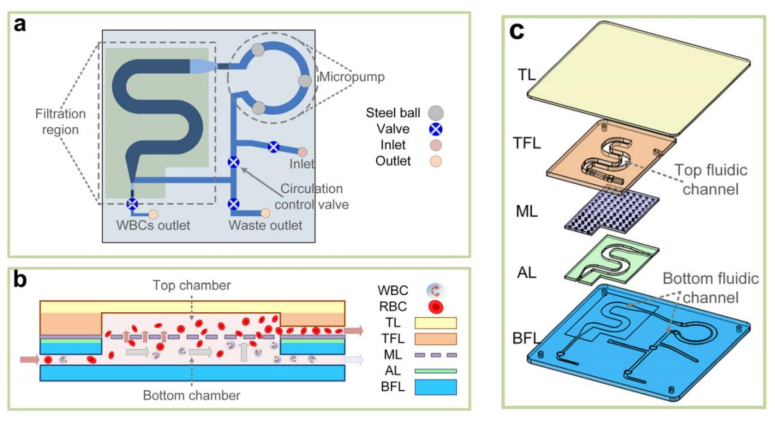
\includegraphics[width=0.8\textwidth]{figures/literaturereview/figure2_1}%
\caption{(a) Schematic of the microfiltration chip. (b) Cross-section of the chip in the filtration region. (c) Explosive view of the multilayer structure of the chip, starting from the bottom: bottom fluidic channel layer (BFL), adhesive layer (AL), Polycarbonate micro-porous membrane layer (ML), top fluidic channel layer (TFL), and top PDMS membrane layer (TL) \cite{cheng2016high}.}%
\label{figure2_1}%
\end{figure}

Cheng et al. \cite{cheng2016high} in 2015 have presented a high-throughput and clogging-free microfluidic filtration platform for on-chip cell separation from undiluted whole blood. This microfluidic platform was designed specifically for rapid separation of white blood cells (WBC) from whole blood sample for point-of-care blood pretreatment and diagnosis applications. Based on polycarbonate micro-porous membrane the white blood cells are separated with cross-flow filtration by driving the sample blood flow over the micro-porous membrane back and forth. \autoref{figure2_1} shows the schematic design of the microfiltration chip and its explosive view. This chip is composed of a micropump, which serves as the driving force of the flow, filtration region where the micro-porous membrane lays, product and waste harvesting interfaces and four valves which are used to change flow direction.

\begin{figure}[ht]%
\centering
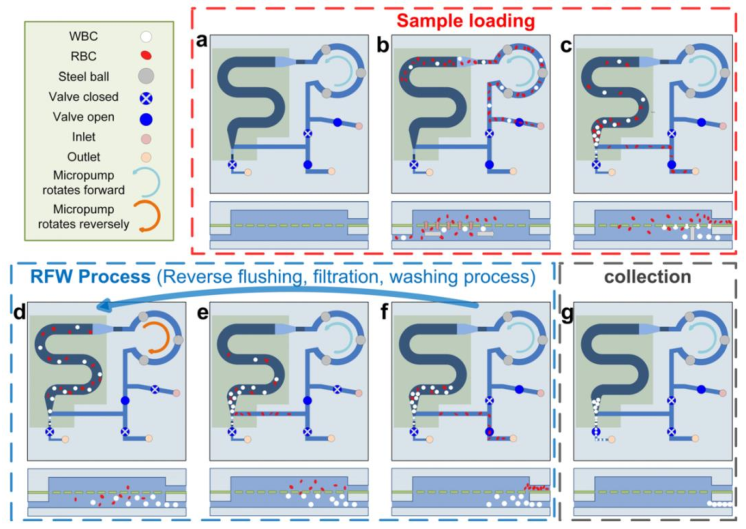
\includegraphics[width=0.9\textwidth]{figures/literaturereview/figure2_2}%
\caption{Working procedures for cell separation. (a) Load buffer. (b) Load whole blood. (c) Load buffer. (d) Reverse flushing. (e) Circulating filtration. (f) Washing away remaining red blood cells and platelets. (g) Collect white blood cell sample \cite{cheng2016high}.}%
\label{figure2_2}%
\end{figure}

The cell separation starts with sample loading, in which a volume of buffer is loaded via the inlet to rinse the chip (\autoref{figure2_2} (a)), followed by a volume of whole blood sample (\autoref{figure2_2} (b)) and then another volume of buffer (\autoref{figure2_2} (c)). Then the fluid is driven by the micropump to flow forward (counterclockwise), during which the whole blood is transported to the filtration region, where white blood cells are stopped by the micro-porous membrane and red blood cells and platelets pass through the membrane and they are harvested at the corresponding outlet. The valves are then adjusted and the micropump changes working direction to drive the fluid to flow backward (clockwise) to repeat the filtration process. This back and forth filtration process will continue working until the filtration is satisfactory. The buffer fluid acts as cleaning flow to flush away the cells trapped in micro-pores in the membrane in order to avoid blocking of the membrane.\\

Another microfluidic platform example presented by Metz et al. \cite{metz2003polyimide} is integrated with nanofiltration membranes for the application of selective delivery or probing of fluids to biological tissue (\autoref{figure2_3}). Based on cross-flow filtration specified particles in the solution can be filtered under pressure generated by a syringe pump. In the former example shown in \autoref{figure2_1} the filtration area is increased by designing the snake-shaped channel. Likewise, Metz designed microchannel structures to intensify the filtration process by increasing the contact area with meander channel geometry. 

\begin{figure}[ht]%
\centering
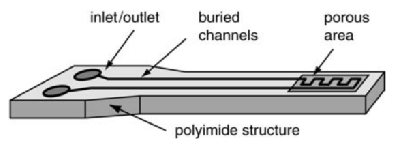
\includegraphics[width=0.5\textwidth]{figures/literaturereview/figure2_3}%
\caption{Schematic of the microchannel design for the nanofiltration process \cite{metz2003polyimide}.}%
\label{figure2_3}%
\end{figure}

\section{Laser Cutting Technology and Silicone Processing Technique}
\label{2_2}
\subsection{Laser Cutting Technology}
\label{2_2_1}

\begin{figure}[!b]%
\centering
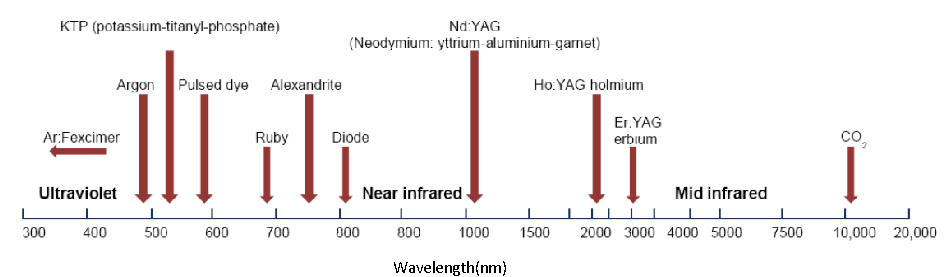
\includegraphics[width=1\textwidth]{figures/literaturereview/figure2_4}%
\caption{Classification of lasers according to the laser wavelength \cite{simpson2012basic}.}%
\label{figure2_4}%
\end{figure}

Laser cutting is now a widely used processing technique and it is more and more competitive over the conventional mechanical processing techniques. Since microstructure construction is always necessary for microfluidic applications, laser cutting has shown its ability in processing structures within the micrometer range and thus became a popular method in MEMS labs. Besides, the high processing efficiency and its processing accuracy are also satisfactory. Based on wavelength lasers can be classified into different types as shown in \autoref{figure2_4}. 

The processing mechanisms of the lasers are not always the same, depending on the laser wavelength. The mechanism of deep ultraviolet (DUV) laser ablation is a photochemical process in which the chemical bonds in the material are broken and fragments thus formed are ejected in plasma plume \cite{lasermicromachining}. Different from that, the infrared or visible lasers such as CO$_2$, Nd:YAG lasers produce fast-heating and melting of the material directly. Specifically when metal foils are processed by these lasers, the laser radiation is absorbed by the work piece within a thin surface layer, which causes a stimulation of bonded electrons and a heating of the free electrons by inverse bremsstrahlung.  Thereby the absorbed energy is deposited into the electron system and is subsequently transferred into the lattice by electron-phonon coupling, leading to the breakup of the atomic and molecular bonds and the expansion of the material (causing melting and evaporation) \cite{ref_4}. 

\begin{figure}[!b]%
\centering
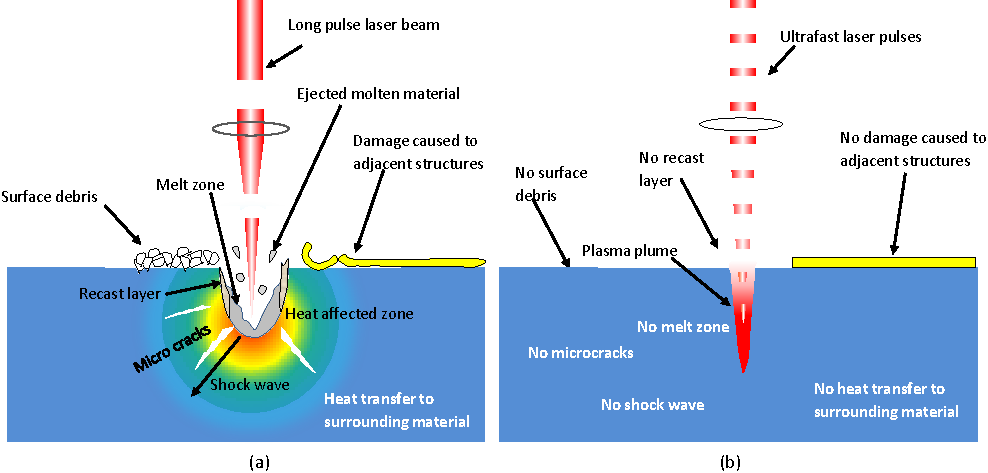
\includegraphics[width=1\textwidth]{figures/literaturereview/figure2_5}%
\caption{Comparison of processing mechanism of long pulse lasers and ultrafast pulse lasers.\cite{ref_4}}%
\label{figure2_5}%
\end{figure}

For the laser ablation process, the pulse length is an essential parameter and lasers can also be classified according to their pulse duration: long pulse lasers (pulse duration longer than 10 picoseconds) and ultrafast pulse lasers (pulse duration less than 10 picoseconds). In the long pulse regime, heat diffusion, melting and material expansion during the laser pulse are considerable. Since the laser pulse duration is longer than the heat diffusion time, the heat generated by the laser radiation will diffuse away to the surrounding area, leading to collateral damage to the surrounding area as shown in \autoref{figure2_5} (a) \cite{ref_4}. This heat diffusion also reduces the efficiency of the micromachining progress since it takes energy away from the work spot -- energy that would otherwise go into removing the material in the work piece. Besides, the absorption of long laser pulse leads to melting and evaporation of the material which can contaminate the surrounding area, produce micro-cracks and remove material over dimensions which are desired. Unlike the long pulse machining, within a ultrafast laser pulse the heat deposited by the laser into the material does not have time to move away from the work spot during the time the laser pulse is illuminating the material (\autoref{figure2_5} (b)) \cite{ref_4}. Therefore the energy is fully absorbed by the material and thus the material is converted from a solid state directly to a gas phase without first going through a melt phase, taking away almost all the heat with it. Consequently, very little heat is left behind to damage the material, thus providing much better processing accuracy than the long pulse lasers \cite{chichkov1996femtosecond}.

\subsection{Silicone Processing Technique}
\label{2_2_2}
Silicones are known as polymers that include any inert, synthetic compound made up of repeating units of slogans, which is a chain of alternating silicon atoms and oxygen atoms, frequently combined with carbon and/or hydrogen \cite{moretto2000silicones}. PDMS, widely used in cleanrooms for the process of soft lithography, is a well-known silicone. Silicones exhibit many useful characteristics including low thermal conductivity, low chemical reactivity, low toxicity, thermal stability, electrical insulation properties. These characteristics make silicones useful in many products, especially for medical applications due to its low chemical reactivity and low toxicity. Many of elements in the microfluidic devices are also made of slickness, leading to many kinds of silicone processing technologies.\\

\begin{figure}[h]%
\centering
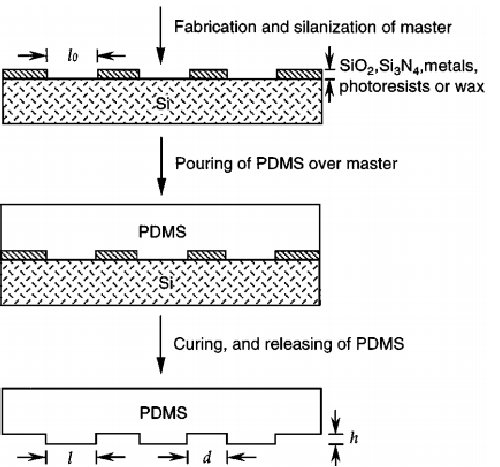
\includegraphics[width=0.6\textwidth]{figures/literaturereview/figure2_6}%
\caption{Fabrication of the PDMS stamp or mold \cite{xia1998soft}.}%
\label{figure2_6}%
\end{figure}

The mainstream microfabrication technology for patterning silicones is soft lithography. Xia et al. presented their soft lithography technology for patterning different geometries of microstructures \cite{xia1998soft}. The key element of soft lithography is an elastomeric block with patterned relief structures on its surface and this element acts as the stamp or mold for the mass fabrication of silicone microstructures. \autoref{figure2_6} shows the procedure for fabricating PDMS stamps from a master having relief structures on its surface. The master is rigid and fabricated using microlithographic techniques such as photolithography or e-beam writing.  After the fabrication and silanization of the master, liquid PDMS is poured over the master and makes conformal contact with the surfaces, forming a patterned PDMS stamp or mold after curing. 

\begin{figure}[h]%
\centering
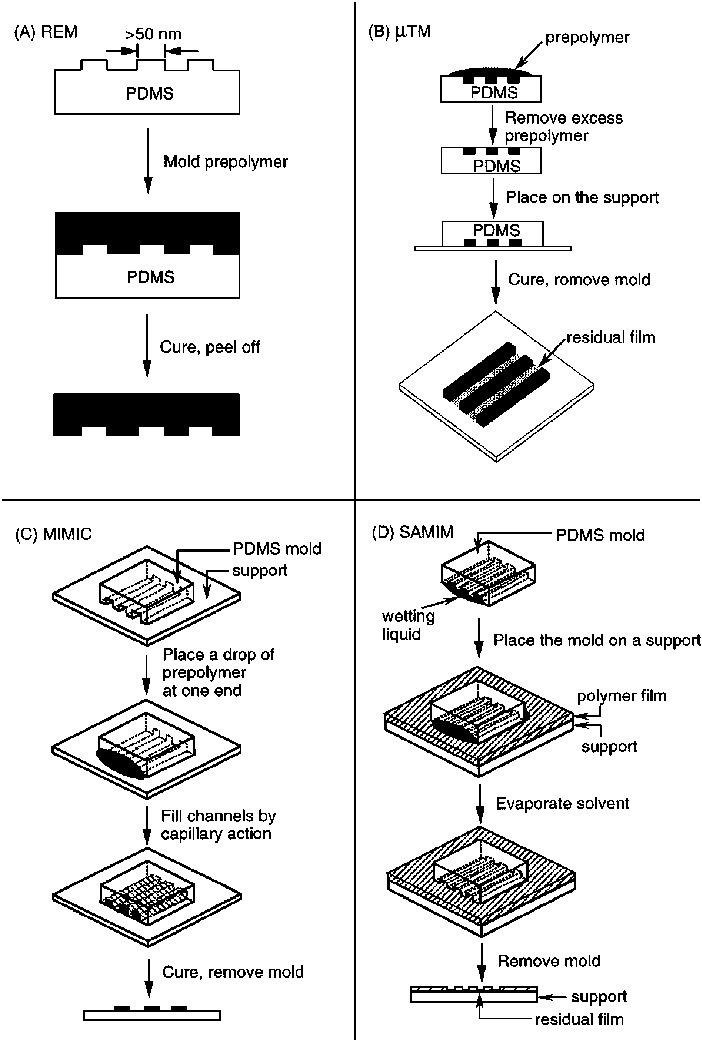
\includegraphics[width=0.65\textwidth]{figures/literaturereview/figure2_7}%
\caption{Schematic illustrations of procedures for (a) Replica Molding (REM), (b) Microtransfer Molding ($\mu$TM), (c) Micromolding in Capillaries (MIMIC), and (d) Solvent-assisted Micromolding (SAMIM) \cite{xia1998soft}.}%
\label{figure2_7}%
\end{figure}

Based on this silicone mold several techniques have been developed by Xia for the mass-producing of microstructures. \autoref{figure2_7} (a) shows the procedure of Replica Molding (REM) technique. The liquid silicone is casted to the PDMS mold and is peeled off after curing. The structures in this silicone are complementary to those on the PDMS mold and are the same to those on the original master. \autoref{figure2_7} (b) shows the procedure of Microtransfer Molding ($\mu$TM) technique. A thin layer of liquid prepolymer is applied to the patterned surface of a PDMS mold and the excess liquid is removed. This mold, filled with the prepolymer, is then placed in contact with the surface of a substrate. The prepolymer is then cured to solid and forms the microstructure on the surface of the substrate when the mold is peeled away. \autoref{figure2_7} (c) presents the Micromolding in Capillaries (MIMIC) technique. In MIMIC a PDMS mold is placed on the surface of a substrate to form empty channels between them and a low-viscosity prepolymer is then placed at the open ends of the channels. This liquid then fills the channels by capillary action and after curing the patterned microstructures are revealed by removing the PDMS mold. In \autoref{figure2_7} (d) the Solvent-Assisted Micromolding (SAMIM) technique is presented. SAMIM generates relief structures in the surface of a material using a good solvent that can dissolve the material without harming the PDMS mold. The PDMS mold is wetted first with the solvent and brought into contact with the surface of the substrate. The solvent then dissolves a thin layer of the substrate. The patterned relief structure complementary to that in the surface of the mold is then formed when the solvent dissipates and evaporates.

\begin{figure}[h]%
\centering
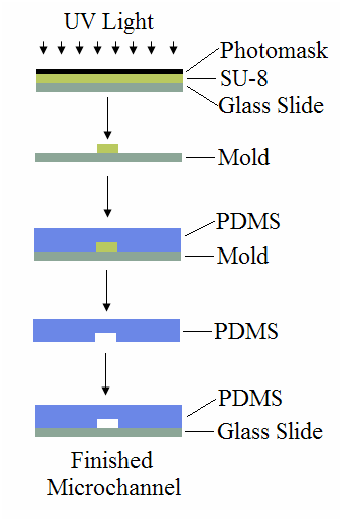
\includegraphics[width=0.4\textwidth]{figures/literaturereview/figure2_8}%
\caption{Schematic for microchannel fabrication procedure \cite{boyajian2010microchannel}.}%
\label{figure2_8}%
\end{figure}

Likewise, Boyajian has presented a similar technique specifically for microchannel \cite{boyajian2010microchannel}. \autoref{figure2_8} shows the schematic procedure for the microchannel fabrication. The master mold is fabricated also by soft lithography technique. The SU-8 photoresist is spin-coated on top of a glass slide and then is covered by photomask. The photoresist is then patterned by UV light exposure and liquid PDMS silicone is poured on top of the mold to the desired thickness. After curing, the PDMS is peeled off of the mold and is bonded to a new glass slide and the microchannel is formed.

\section{Sealing and Packaging of High Pressure Microfluidic Systems}
\label{2_3}
To ensure the reusability and resealability for high pressure microfluidic applications, the sealing and packaging technology of the device is still a significant technical challenge. There are several sealing and packaging processes that can be summarized into two main categories: permanent sealing and nonpermanent sealing. Permanent sealing can be realized by a lot of different bonding and gluing processes and is widely used in microfluidic devices. Nonpermanent sealing is realized by applying O-rings or only by conformal contact. For the application in this thesis work, nonpermanent sealing technique is required since the microfluidic platform should be resealable and reusable for the integration of many different membrane samples.\\

\begin{figure}[!b]%
\centering
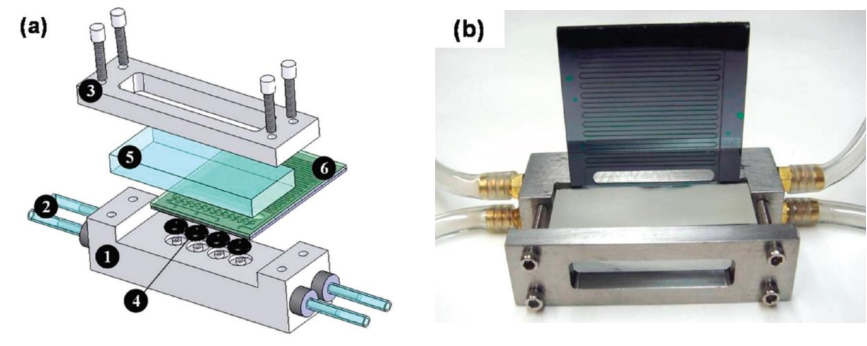
\includegraphics[width=0.8\textwidth]{figures/literaturereview/figure2_9}%
\caption{(a) Scheme of a high pressure microfluidic assembly: (1) compression part, (bottom) with modular fluidics inlet/outlet ports, (2) cooling fluid pathway, (3) compression part (top), (4) O-rings and grooves, (5) Pyrex plate for optical access, (6) microreactor. (b) Image of the final assembly \cite{marre2010design}.}%
\label{figure2_9}%
\end{figure}

Marre et al. \cite{marre2010design} in 2010 has presented a sealing method for high pressure and high temperature microreactors. For easy fabrication and easy interchange of microreactors, nonpermanent connections based on the compression of O-rings are applied. \autoref{figure2_9} shows the scheme of the microreactor assembly. The compression chuck consists of two stainless steel parts compressing the microreactor (part 1 and part 3 in \autoref{figure2_9} (a)). The bottom one is integrated with tubes (part 2) for the cooling of the microreactor while the upper part aims at compressing the microreactor against O-rings (part 4) and holding pressure. The upper part is equipped with a window for visualization of the microreactor. Therefore in order to ensure good homogeneity in the compression, an additional Pyrex part (part 5) is placed in between the microreactor and the upper part.

While nonpermanent sealing provides great convenience for the resealability and reusability of the microfluidic device, the pressure it can withstand is not always as high as certain permanent connection methods. Therefore adhesive assisted sealing or bonding techniques presents in most of the microfluidic devices. Li et al. \cite{li2014usb} have presented an adhesive based sealing technique for developing microfluidic chips on printed circuit boards (PCB) as shown in \autoref{figure2_10}. This microfluidic chip is fabricated on PCB in order to provide fast monitoring of the flow and a more compact integration. The geometry of the microchannel is at first designed and printed to the copper layer of PCB by standard PCB etching technology. The fabricated PCB is then covered by a glass slide, which is coated with a UV-curable adhesive. The microchannels are completed after the UV solidification of the adhesive.

\begin{figure}[ht]%
\centering
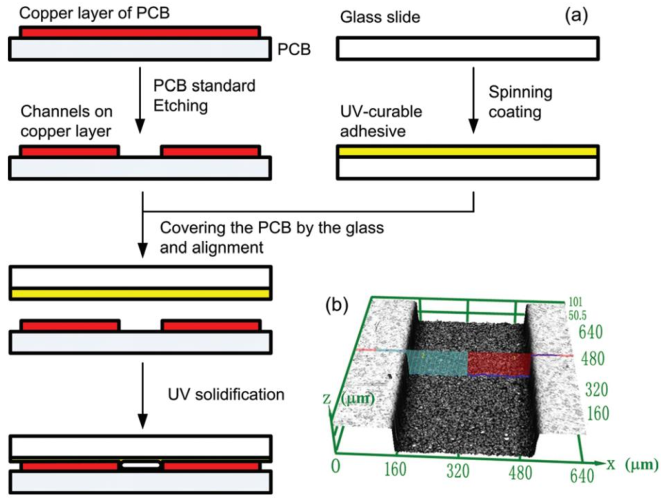
\includegraphics[width=0.7\textwidth]{figures/literaturereview/figure2_10}%
\caption{(a) Fabrication process of the microchannels on a PCB. (b) 3D topography of a fabricated microchannel on a PCB \cite{li2014usb}.}%
\label{figure2_10}%
\end{figure}












